\chapter{Supporting Materials}

\section{Increased \acs*{abmd} due to larger bone size}
\label{sec:support_abmd}
This section explains the effect of larger bone size on \ac{abmd} discussed in \S\ref{sec:fractures_clinic_risk}.

Areal bone mineral density (\acs{abmd}) can be artificially increased if the bone being scanned in a \acf{dxa} scanner is larger than assumed (\ac{ie}, larger than the reference population).
For example, consider a vertebral body to be cylindrical in shape.
If the diameter and height of the reference population vertebra are 2~\ac{cm} each, the volume would be 12.56~\ac{cm}$^3$, and the projected area would be 4~\ac{cm}$^2$.
Now consider that the reference population \ac{bmd} is 2~\ac{g}/\ac{cm}$^3$, so the total \ac{bmc} is 12.56~\ac{g}, and the \ac{abmd} would be $($12.56~\ac{g}$/$4~\ac{cm}$^2)$ = 3.14~\ac{g}/\ac{cm}$^2$.
If we now consider a large patient whose vertebra has a diameter and height of 3~\ac{cm} each, they would have a total volume of 21.2~\ac{cm}$^3$, and a projected area of 9~\ac{cm}$^2$.
If this patient has the same \ac{bmd} of 2~\ac{g}/\ac{cm}$^3$, they would have a total \ac{bmc} of 42.4~\ac{g}, and an \ac{abmd} of 4.71~\ac{g}/\ac{cm}$^2$, indicating that the larger patient has 50\% more dense bone, even though their \ac{bmd} was the same.

\section{Femoral neck internal rotation justification}
\label{sec:support_orientation}
Femoral orientation in the fall protocol defines the position of the femoral neck as 15$^\circ$ internal rotation.
This value can be shown to be approximately correct using data from \citet{toogood_proximal_2009} and \citet{feldman_reducing_2007}.
\citet{feldman_reducing_2007} reported a ``hip proximity angle" of approximately 8$^\circ$ posterior.
This angle is referenced to the centre of the pelvis, and is a different angle when referenced to the centre of the femoral head (Figure~\ref{fig:hipProximity}).

\begin{figure}
	\centering
	\includegraphics[width=1\linewidth]{./appendixSupport/Figures/hipProximity}
	\caption[Hip proximity related to femoral head]{\textbf{The hip proximity angle is referenced to the centre of the pelvis. Changing the reference to the centre of the femoral head roughly doubles the angle}. Graphic adapted from \citet{inversitus_prostatic_2012}, permission not required.}
	\label{fig:hipProximity}
\end{figure}

Assuming that the femoral head lies approximately one third of the way from the centre of the pelvis to the surface of the hip, a hip proximity angle of 8$^\circ$ gives an angle of approximately 22.9$^\circ$ degrees when referenced to the femoral head (Equation~\ref{equ:hipProx}).
\vspace{-1EX}
\begin{eqnarray}
\tan(\alpha) &=& \frac{x}{L}  \nonumber \\
\Leftrightarrow x &=& L \cdot \tan(\alpha)\nonumber \\
\tan{\beta} &=& \frac{x}{L/3}\nonumber \\
\Leftrightarrow \tan{\beta} &=& \frac{L \cdot \tan(\alpha) }{L/3}\nonumber \\
\therefore \beta &=& \arctan(3 \cdot \tan(\alpha))\nonumber \\
\Leftrightarrow \beta &=& \arctan(3 \cdot \tan(8^\circ)) = 22.9^\circ
\label{equ:hipProx}
\end{eqnarray}

The impact angle of 22.9$^\circ$ internal rotation about the femoral head is independent of femoral twist, which tends to decrease the value of the impact angle.
The femoral twist in the normal population is 9.73$^\circ$~\citep{toogood_proximal_2009}, so the resulting average impact angle would be 13.1$^\circ$.
This is not the value of 15$^\circ$ used in the research, but given the impact angle standard deviation of 15$^\circ$, and femoral twist angle standard deviation of 9.28$^\circ$, the standard orientation is well within the expected normal variation.

\section{Calculation of Mass 1 initial velocity}
\label{sec:support_mass1_velocity}
The velocity of Mass 1 in the idealized model discussed in \S\ref{sec:behave_fail_discssion} can be calculated as shown below.
\vspace{-1EX}
\begin{eqnarray}
E_{start} &=& E_{finish}\nonumber \\
E_{start} &=& \frac{1}{2} \cdot m_{st} \cdot V_{st,start}^2 + \frac{1}{2} \cdot m_{body} \cdot V_{body,start}^2\nonumber\\
E_{finish} &=& \frac{1}{2} \cdot m_{st} \cdot V^2 + \frac{1}{2} \cdot m_{body} \cdot V^2\nonumber\\
m_{st} \cdot V_{st,start}^2 + m_{body} \cdot V_{body,start}^2 &=& \left(\cdot m_{st} + \cdot m_{body}\right) \cdot V^2\nonumber\\
\therefore V &=& \sqrt{ \frac{m_{st} \cdot V_{st,start}^2 + m_{body} \cdot V_{body,start}^2}{m_{st} + \cdot m_{body}} }
\end{eqnarray}

Where $m_{st}$ is the stationary mass of the top plate (1~\ac{kg}) and top $\frac{1}{3}$ of the spring (1.17~\ac{kg}), and $V_{st}$ is the initial velocity of the stationary mass, namely, zero.
Filling in the missing numbers and solving.
\vspace{-1EX}
\begin{eqnarray}
V &=& \sqrt{ \frac{2.17 \cdot 0^2 + 32 \cdot 3^2}{2.17 + \cdot 32} }\nonumber\\
  &=& 2.90\left[m/s\right]
\end{eqnarray}

\section{Equation related to the response of an isolated ideal femur under constant displacement rate loading}
\label{sec:support_courtney_response}
The response of the idealized model of the loading performed by \citet{courtney_effects_1994}, discussed in \S\ref{sec:behave_fail_discssion_relating}, can be calculated using a fixed velocity, and selecting either a maximum displacement or maximum force.
The use of either maximum displacement or force has an affect on the shape of the displacement rate \ac{vs} relative stiffness graph, so explicit selection of this parameter is important.
\vspace{-1EX}
\begin{eqnarray}
F &=& ks + c\dot{s} \nonumber\\
k_{total} = \frac{F}{s} &=& \frac{ks + c\dot{s}}{s}\nonumber
\end{eqnarray}

Calculating the stiffness up to a set displacement gives a linear relationship with \ac{cdamp} (Equation~\ref{equ:stiff_disp}).
Note that when \ac{cdamp} is high the force at even small displacements can be very high, dominated by the damping portion of the relationship.
This makes calculation of th total stiffness up to a given force, rather than given displacement, preferable.
\vspace{-1EX}
\begin{eqnarray}
k_{Total} = \frac{F_{max}}{s_{max}} &=& \frac{ks_{max} + c\dot{s}}{s_{max}} \nonumber \\
\label{equ:stiff_disp} \therefore k_{Total} &=& k + \frac{c\dot{s}}{s_{max}}
\end{eqnarray}

Calculating the stiffness to a set force gives an inverse relationship with (1 - \acs{cdamp}) (Equation~\ref{equ:stiff_force}).
\vspace{-1EX}
\begin{eqnarray}
k_{Total} = \frac{F_{max}}{s_{max}} &=& \frac{ks_{max} + c\dot{s}}{s_{max}} \nonumber \\
s_{max} &=& \frac{F_{max} - c\dot{s}}{k} \nonumber \\
\therefore k_{Total} &=& \frac{k\left( \frac{F_{max} - c\dot{s}}{k} \right) + c\dot{s}}{\frac{F_{max} - c\dot{s}}{k}} = \frac{F_{max}}{\frac{F_{max} - c\dot{s}}{k}} \nonumber \\
\label{equ:stiff_force} k_{Total} &=& \frac{k}{1 - c\frac{\dot{s}}{F_{max}}} 
\end{eqnarray}

\section{Testing log sheets}
\label{sec:support_logsheets}
The following four pages contain the test day log and checklist used to ensure data integrity and communicate with \ac{fe} modellers.
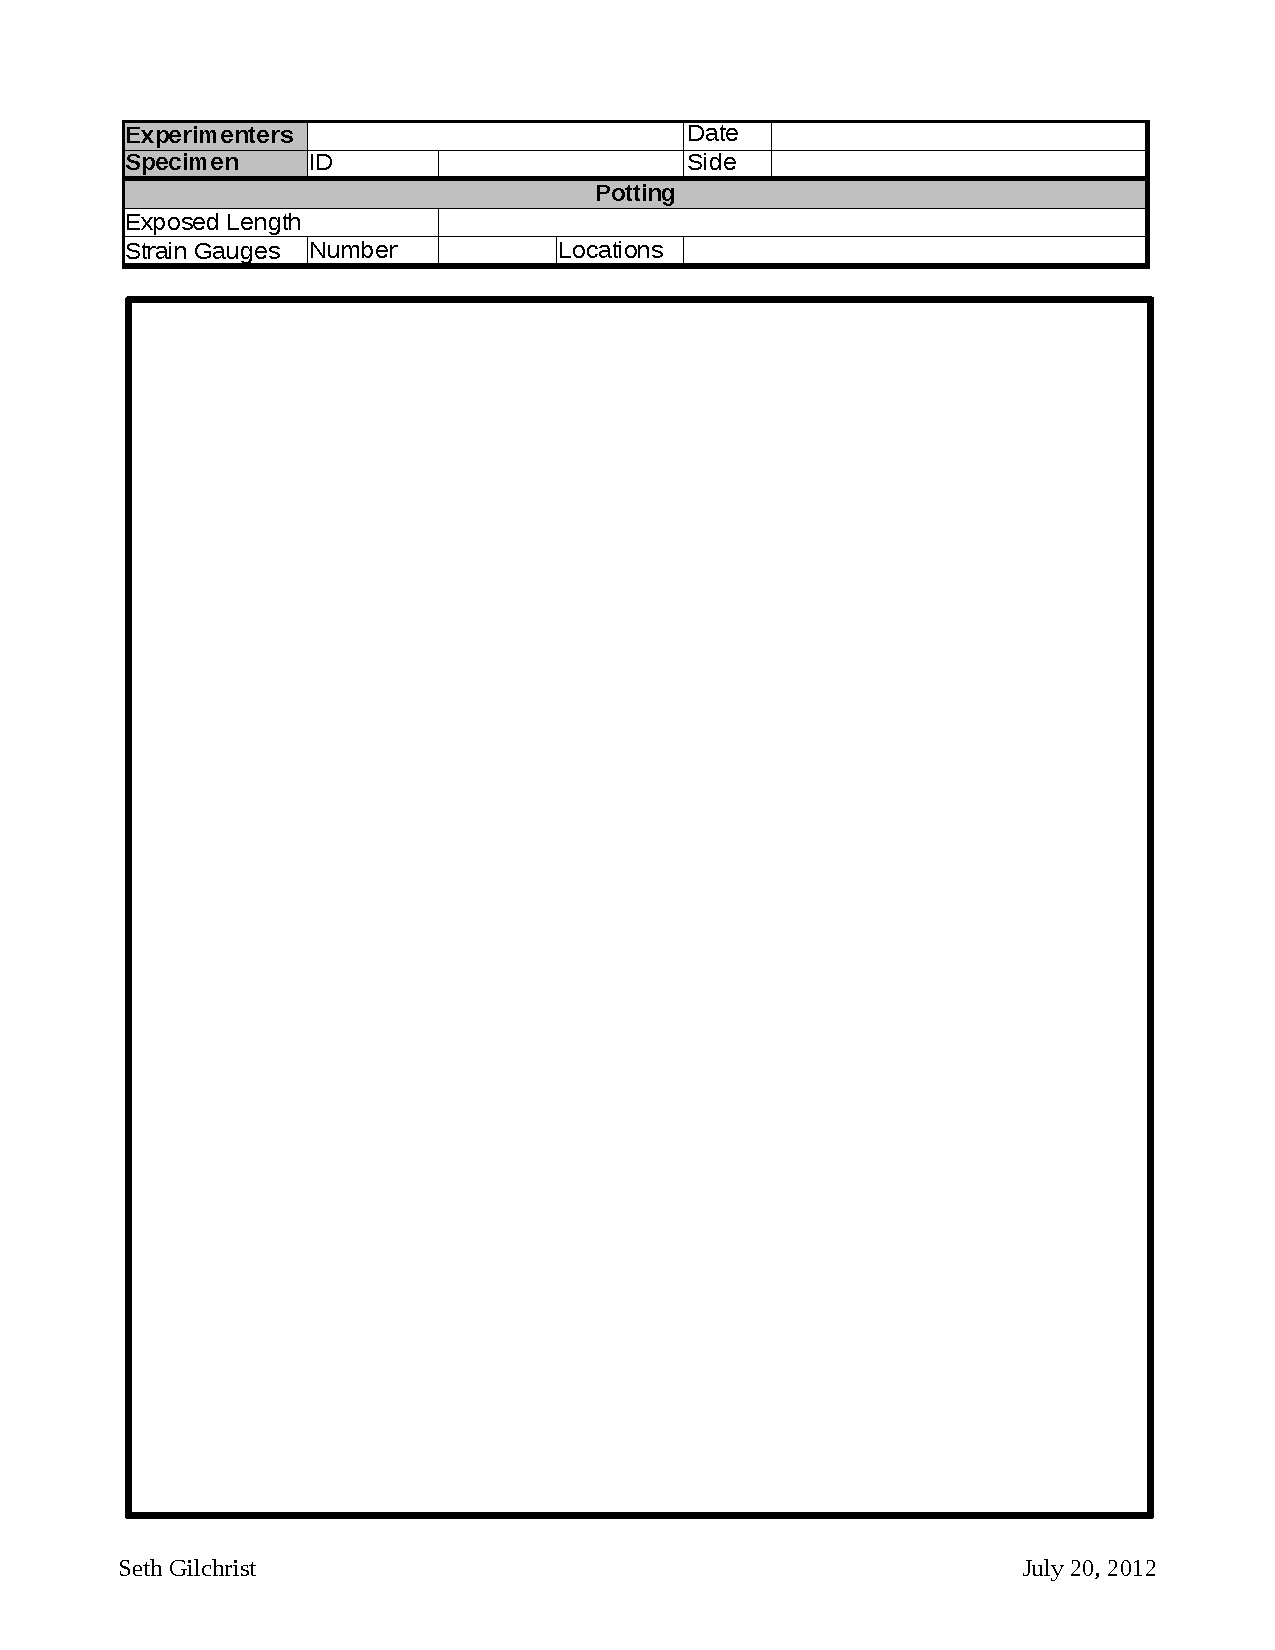
\includepdf[pages={1-4},fitpaper=true,pagecommand=\thispagestyle{plain}]{./appendixSupport/LogSheet.pdf}

\section{Equipment characterization experiments}
\label{sec:equipment}
This section details validation and characterization experiments conducted to ensure data integrity and understand measurement uncertainty.
Each subsection will detail an experimenta and the results of that experiment.

\subsection{Drop tower fall velocity characterization}
\label{sec:equipment_dt_velocity}
The drop tower is a highly constrained, four post design with four in-plane bearings used to direct the gantry.
Due to the constraint of the bearings and posts, the drop tower does not act in free-fall during a drop, but instead must be characterized by a height \ac{vs} impact velocity relationship.
Once this relationship is known the height can be used to anticipate the velocity at impact.

\subsubsection{Method}
The drop tower gantry was loaded with five different masses and dropped from three heights.
Each mass and height was repeated a minimum of two times.
Drops with 32.4~\ac{kg} and 34~\ac{kg} masses were repeated three times at 0.6~\ac{m} as these were lose to the test condition.
The gantry was filmed using a high speed camera (V12.1, Vision Research, Wayne, NJ) at a frame rate of 6200~\ac{fps}, and resolution of 1280x800~\ac{px} (4.8~\ac{px}/\ac{mm}).
The velocity was measured using the time for the drop tower gantry to travel the last inch before contact.
Velocity \ac{vs} drop height was plotted for each mass, additionally, the data at each drop height were combined to generate and average curve for the 29.5-41~\ac{kg} mass range.

\subsubsection{Results}

The drop tower displayed a linear relationship between drop height and velocity (Figure~\ref{fig:dtVelocity}).
The mass had a much smaller influence than the height, however, the single mass below 30~\ac{kg} displayed a lower velocity profile than the other masses.
The average line was highly linear (Equation~\ref{equ:dtVelocity}, $R^2 = 0.9$, $p = 0.015$).
The target velocity for the drops in the experiments was 3.0~\ac{m}/\ac{s}, and from the averaged equation, this lead to a drop height of 62~\ac{cm}.

\begin{equation}
\label{equ:dtVelocity}
Velocity = 2.288 \cdot Height + 1.575
\end{equation}

\begin{figure}
\centering
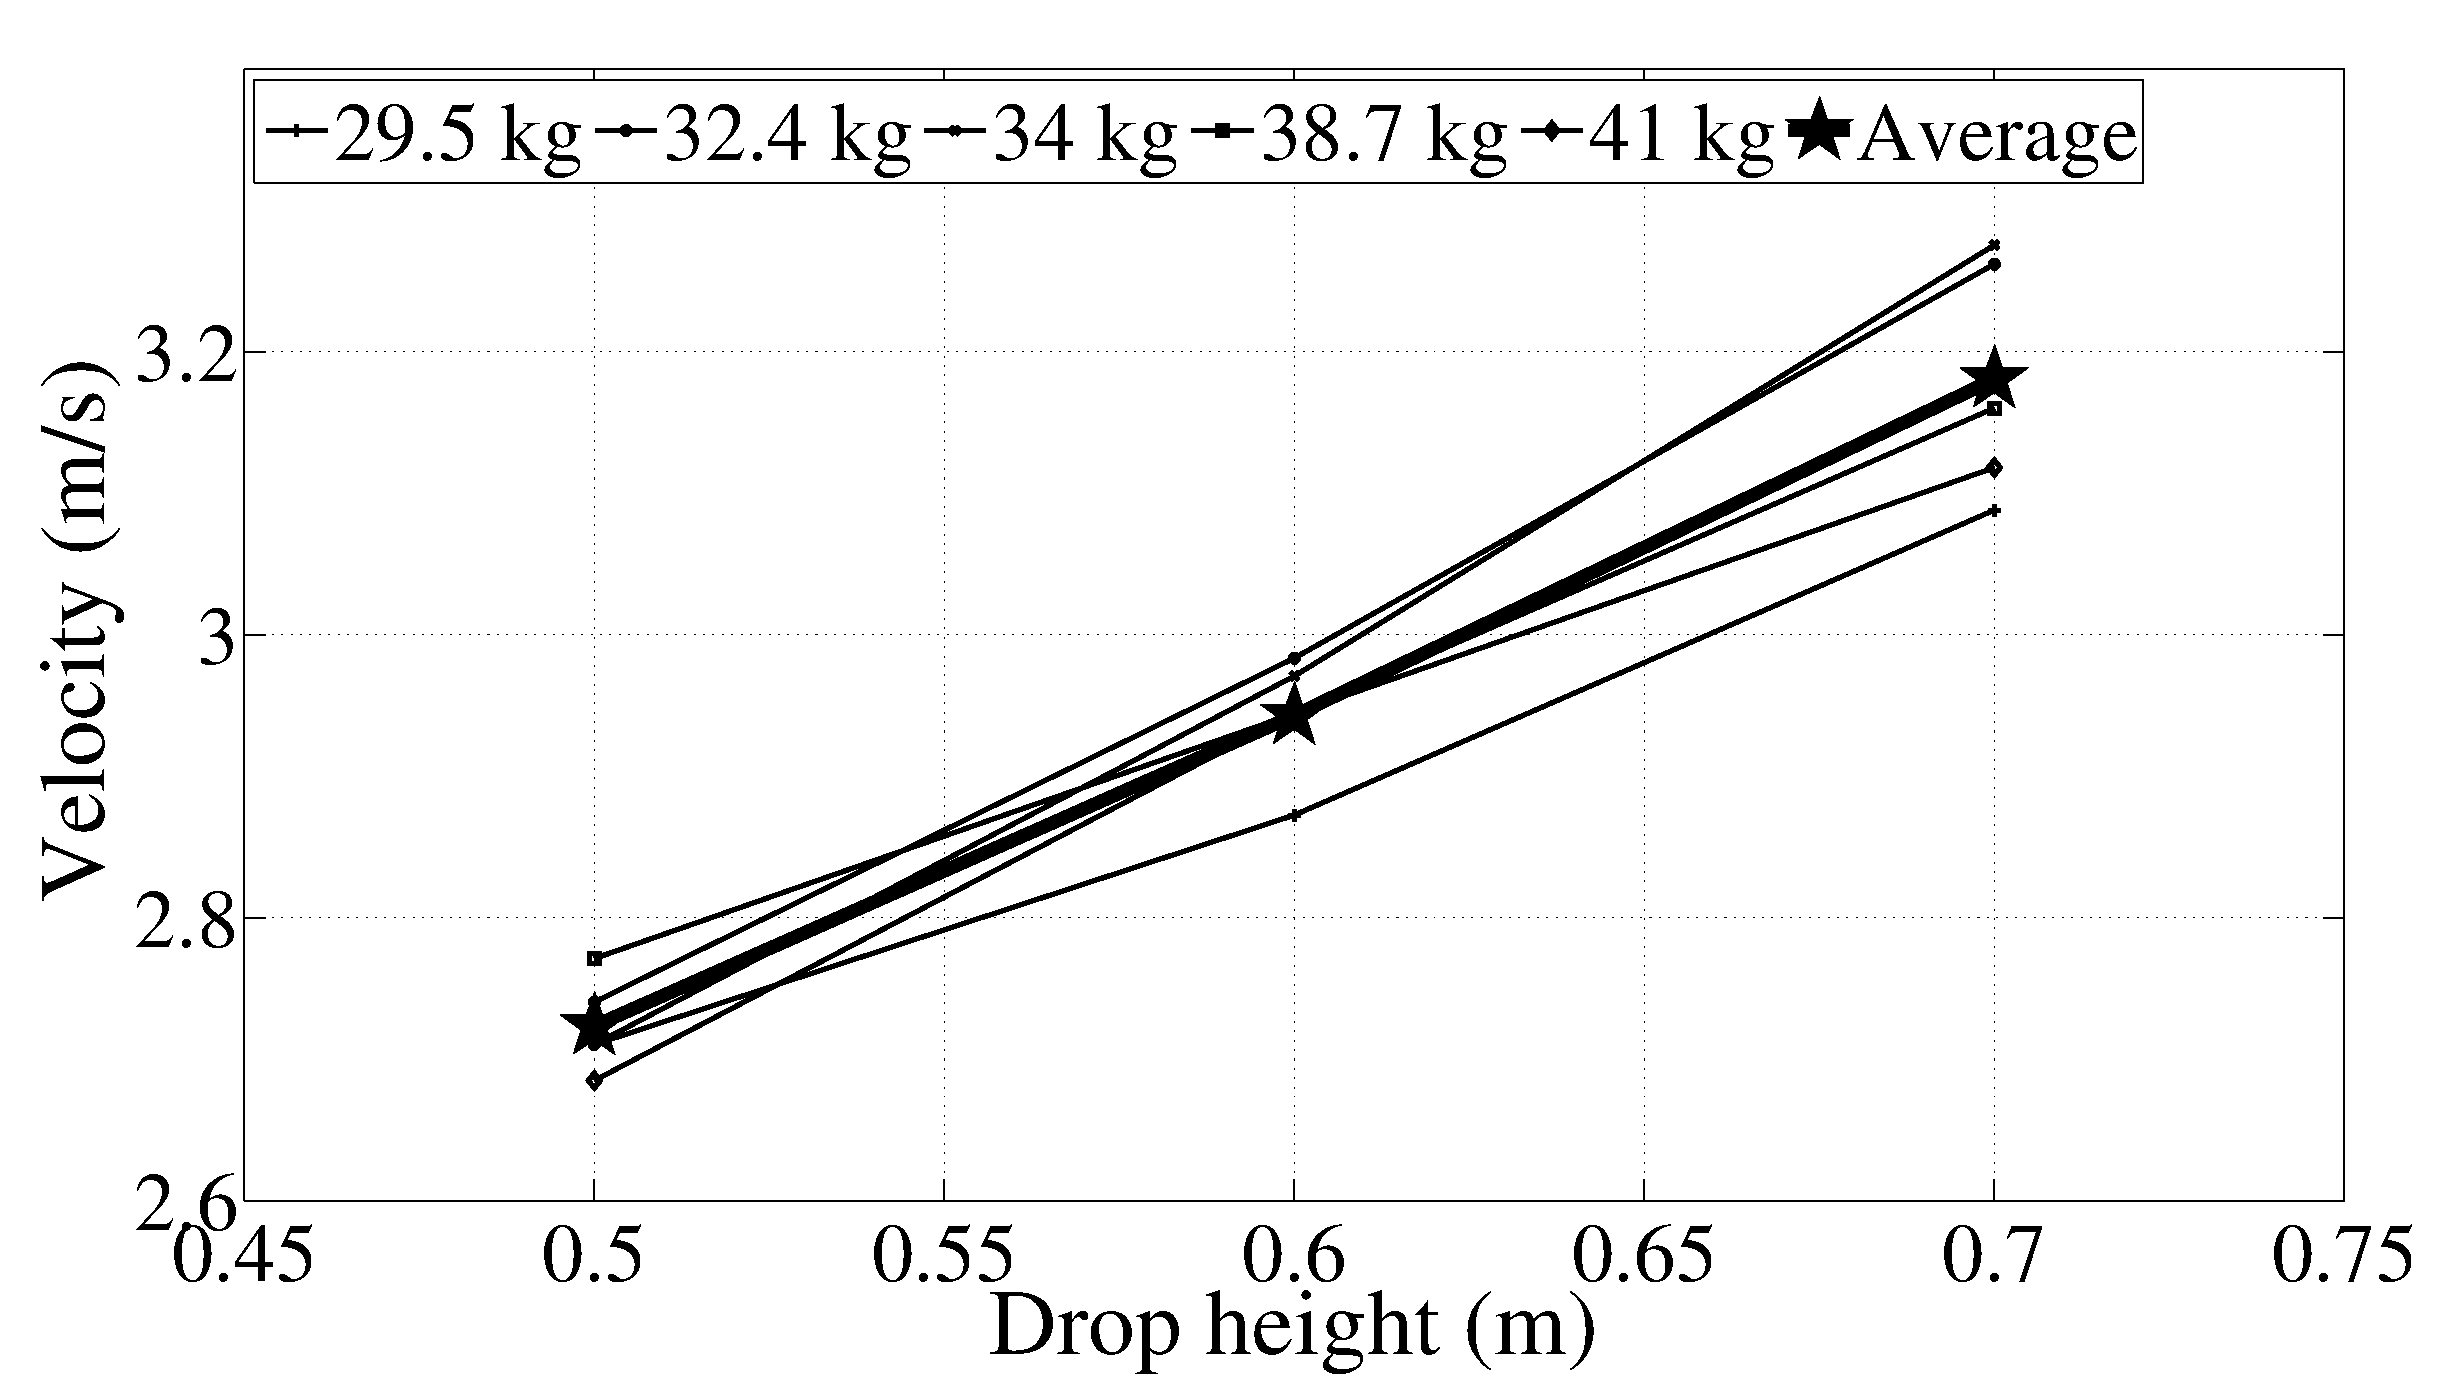
\includegraphics[width=\linewidth]{./appendixSupport/Figures/dtVelocity}
\caption[Drop tower calibration]{\textbf{The drop tower velocity was sensitive to height, and to some degree to mass loaded. At mass $>$30~\ac{kg}, the variation due to mass was irregular.} Graphic \copyright Seth Gilchrist, 2013.}
\label{fig:dtVelocity}
\end{figure}

\subsection{Potting torsion resistance}
\label{sec:equipment_potting}
The method used to pot the specimens was changed to make the potting easier and independent of the mounting apparatus.
Previously, the specimens were potted directly into an aluminium tube that was part of the mounting apparatus.
The new method places the specimens in a 2~inch, schedule 40 \ac{pvc} pipe which is then secured in the testing apparatus using six set screws.
This test was to confirm that the set screws could resist the anticipated torque loads applied during testing.
An instructional video for how to pot the specimens can be found at \url{http://youtu.be/qK967DE0y-Q}.

\subsubsection{Methods}
The torque loads were estimated by mounting a plastic bone replica (v3 large composite femur, Sawbones, Vashon, WA) and taking a measurement from the superior, in the transverse plane from the most lateral point on the greater trochanter to the most medial point on the femoral head.
This measurement was 1.2~\ac{cm}.
The maximum expected load for the femurs was 6000~\ac{n}, leading to a maximum expected torsion of 72~\ac{n}\ac{m}.
A factor of safety of 1.3 was considered acceptable for this torque value, leading to a maximum testing torque of 93.6~\ac{n}\ac{m}, which was rounded up to 100~\ac{n}\ac{m}.

A piece of 1~inch, hexagonal bar with a 3/8~inch tapped hole was potted in the same \ac{pvc} pipe that was going to be used for the testing.
A torque wrench was used to apply torsions of 60, 80 and 100~\ac{n}\ac{m} to a 3/8~inch steel bolt placed in the tapped hole in the hexagonal bar (Figure~\ref{fig:PottingTest}).
Photographs were taken after each torsion to check for rotation of the \ac{pvc} pipe.

\begin{figure}
\centering
\includegraphics[width=\linewidth]{./appendixSupport/Figures/PottingTest}
\caption[Potting torsion resistance]{\textbf{A 3/8~inch bolt was potted in the \ac{pvc} pipe that would be used for testing. A moment was applied to the bolt with a torque wrench and photographs were used to determine if any rotation had taken place.} Graphic \copyright Seth Gilchrist, 2013.}
\label{fig:PottingTest}
\end{figure}

\subsubsection{Results}
Torsion values of 60, 80 and 100~\ac{n}\ac{m} were successfully withstood by the set screws.
Notably, the 3/8~inch bolt yielded at about 98~\ac{n}\ac{m} and 100~\ac{n}\ac{m} was attained only for a short time before the test had to be completed in order to avoid torquing the head off the bolt.

\subsection{Materials testing machine compliance}
\label{sec:equipment_instron_compliance}
Displacements were measured in the materials testing machine using the \ac{lvdt} incorporated in the machine, which measures the ram displacement.
This value will consist of the displacement of the trochanter due to the compression of the bone, as well as the displacement of the trochanter due to translation of the head as the loading plates and bearing plates below the specimen compress.
This tests was conducted to measure the degree that the loading and bearing plates below the femoral head compress during testing.

\subsubsection{Methods}
The test apparatus consists of three ground steel plates with bearing plates between them and two aluminium spacer plates on either side of the specimen (Figure~\ref{fig:InstronCompliance}).
Two pieces of rubber were placed in the space normally occupied by a specimen.
These rubber mats were there to increase compliance and prevent machine overload.
A dial gauge was used to measure the compression of the rubber.
A laser level was used to ensure that the dial gauge probe was perpendicular to the testing machine base.
The cross head of the materials testing machine (8874, Instron, Noorwood, MA) was moved down manually in displacement control until a compressive force of 500~\ac{n} was achieved.
The force was allowed to settle until it was steady within 1~\ac{n} for 60~\ac{s} and the displacement was read.
The compressive force was increased by 500~\ac{n} and the process repeated until a compressive force of 2000~\ac{n} and been achieved.

\begin{figure}
\centering
\begin{subfigure}[b]{0.58\textwidth}
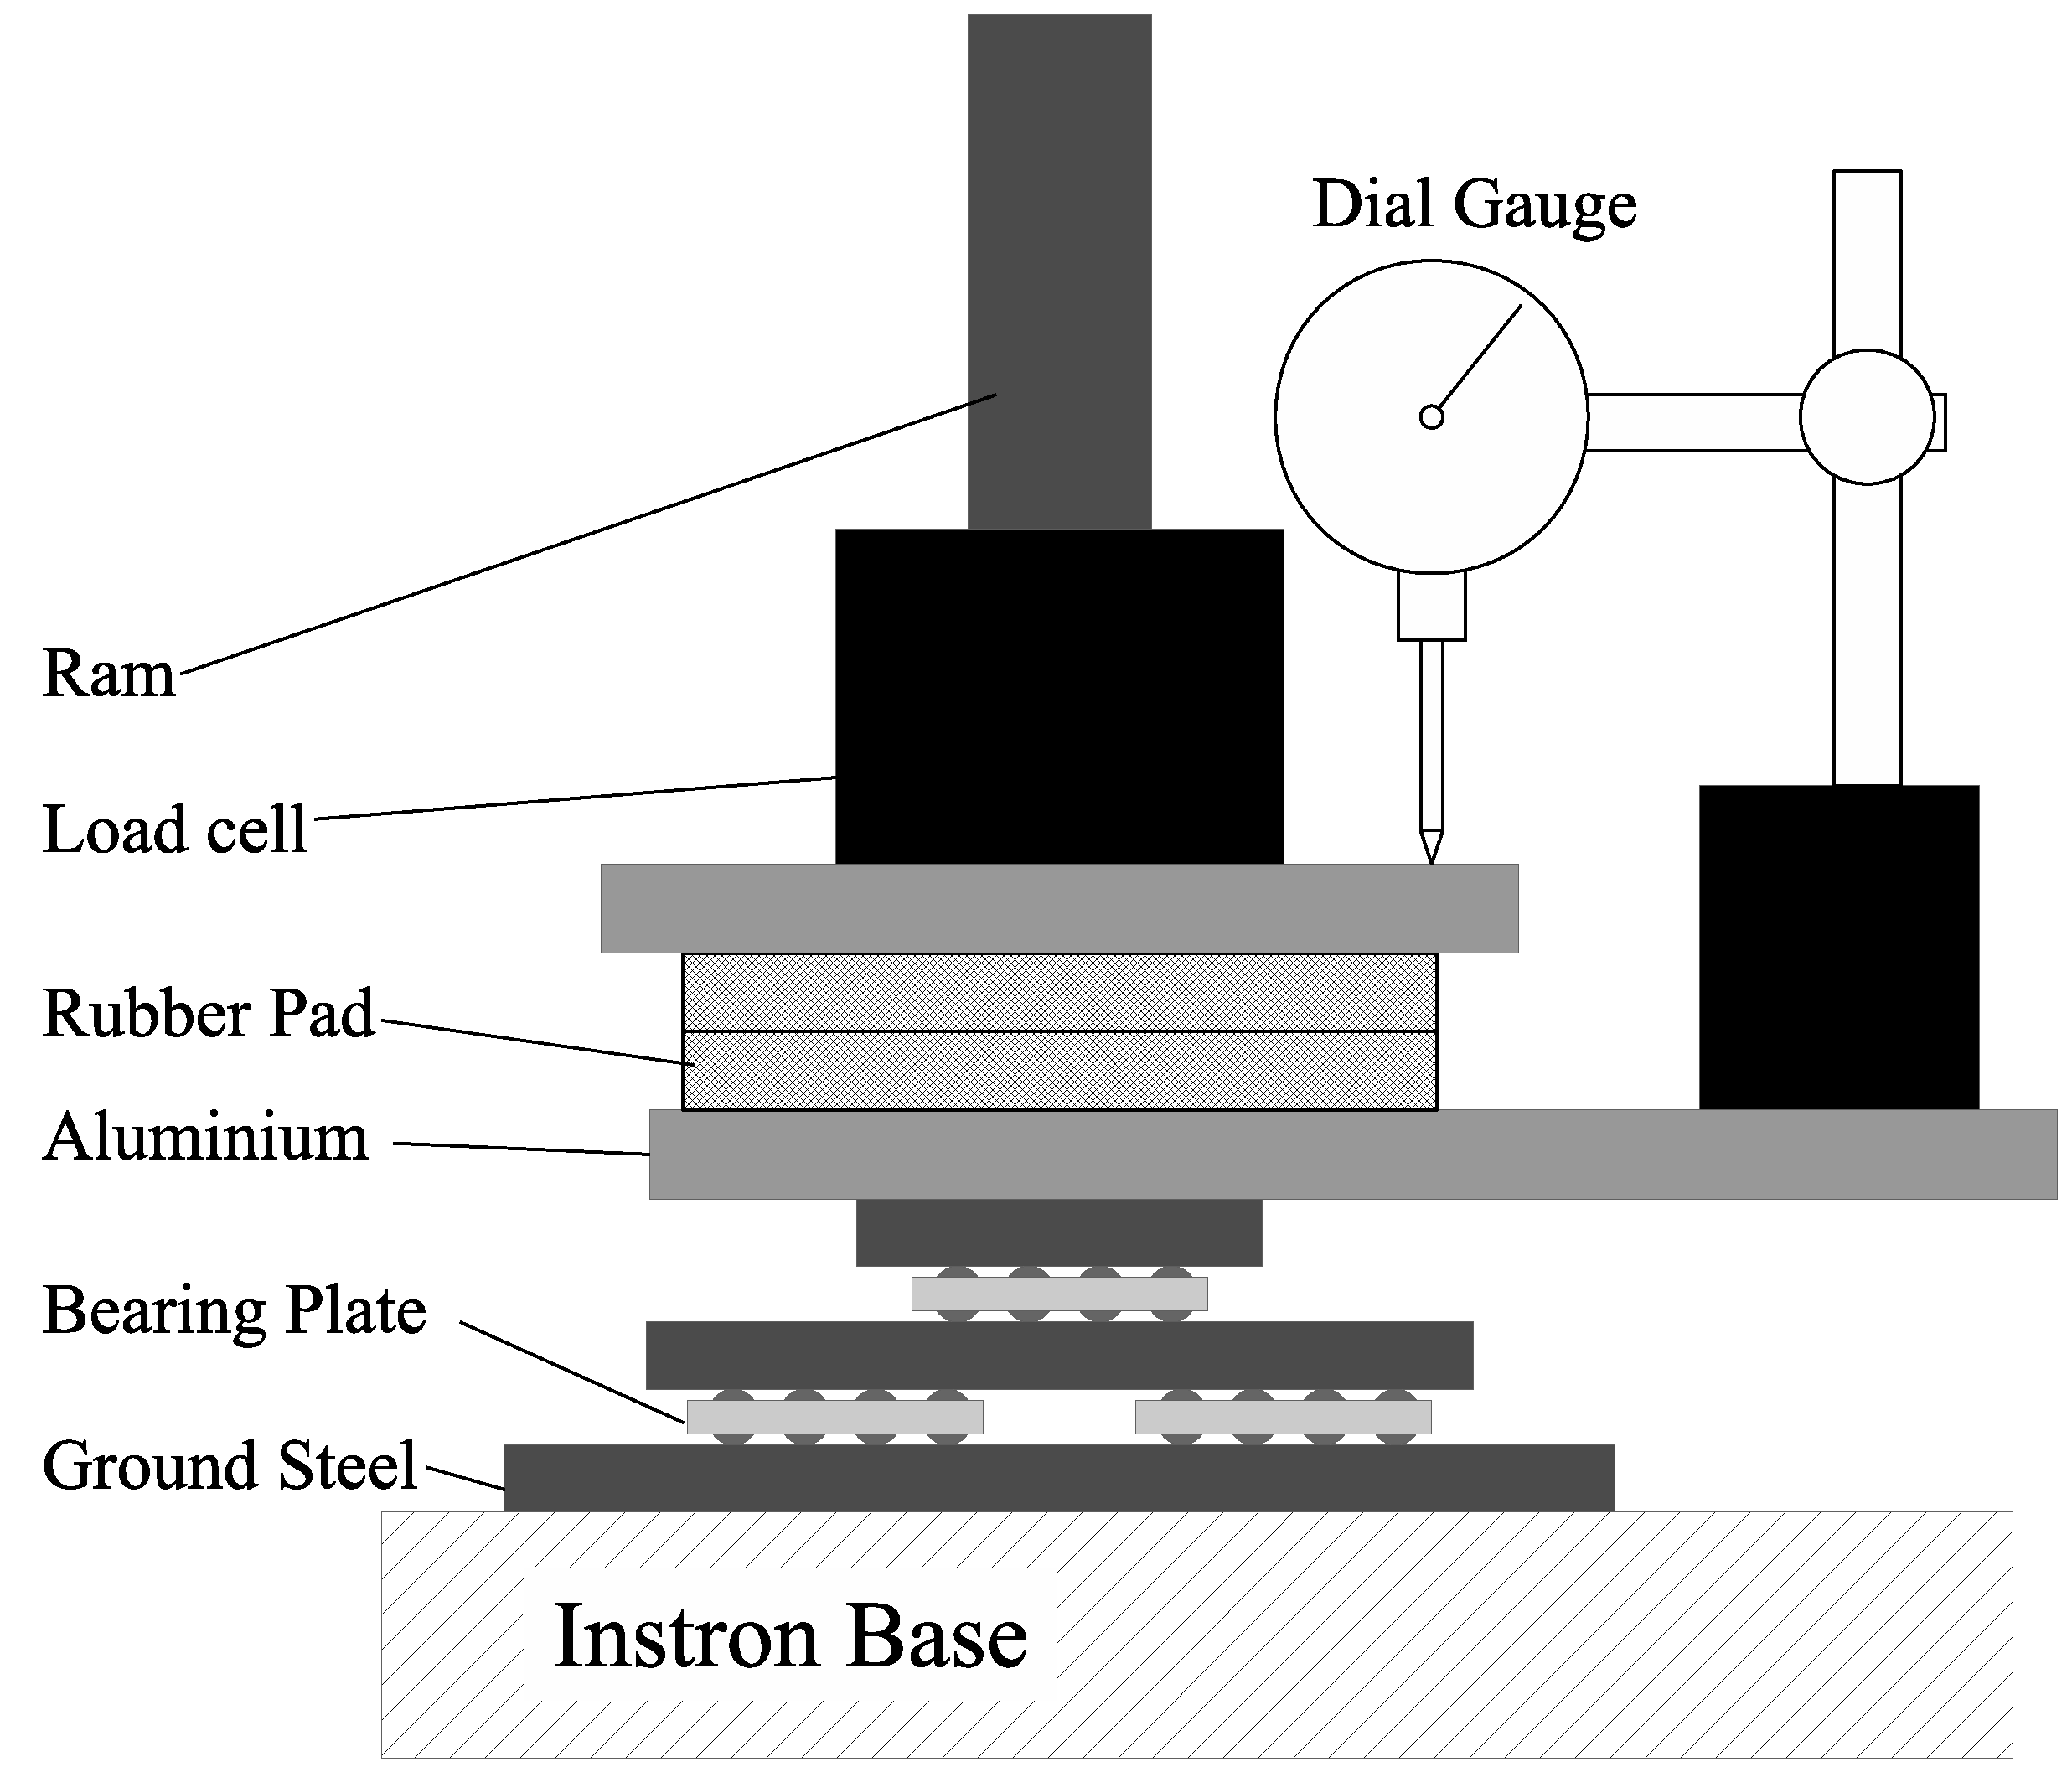
\includegraphics[width=\textwidth]{./appendixSupport/Figures/InstronCompliance}
\caption{Schematic of the loading apparatus}
\label{fig:instronCompSchematic}
\end{subfigure}
~
\begin{subfigure}[b]{0.38\textwidth}
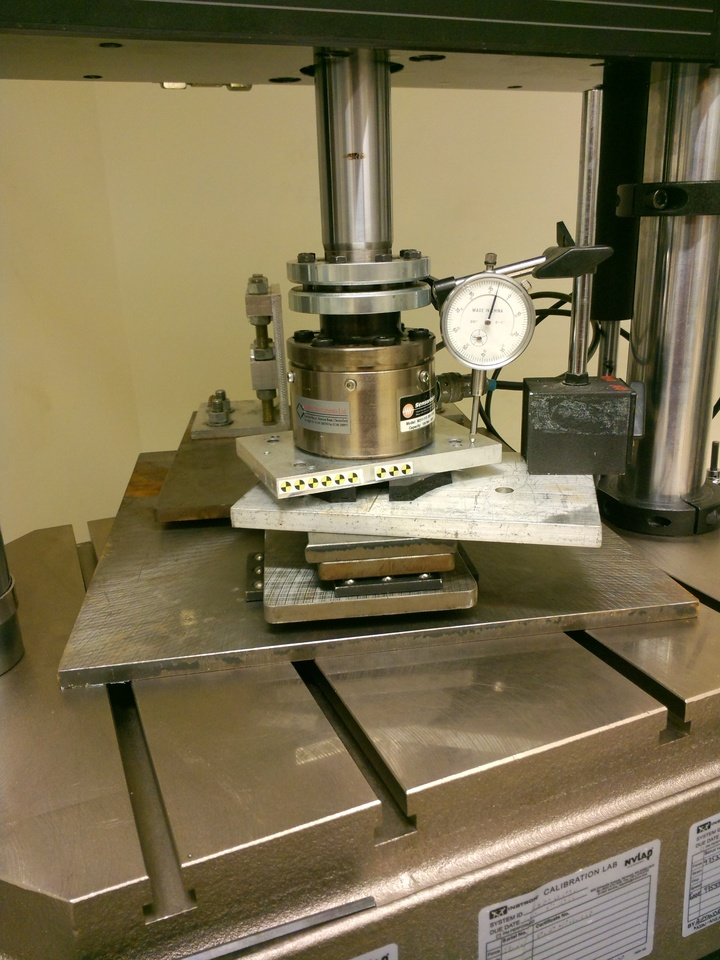
\includegraphics[width=\textwidth]{./appendixSupport/Figures/InstronSetup}
\caption{Photo of the loading apparatus}
\label{fig:instronCompPhoto}
\end{subfigure}
\caption[Materials testing machine compliance test]{\textbf{In the materials testing machine compliance test a rubber mat was compressed in the test apparatus. A dial gauge was used to read the compression of the rubber which was subtracted from the displacement of the load cell to get the compression of the lower plates.} Graphic \copyright Seth Gilchrist, 2013.}
\label{fig:InstronCompliance}
\end{figure}

\subsubsection{Results}
The compression of the apparatus increased linearly with increasing force (Figure~\ref{fig:insComp}).
The stiffness of the bearing plates was found to be approximately 30~\ac{kn}/\ac{mm}, which is about 10-30x that observed for a typical specimen.

\begin{figure}
\centering
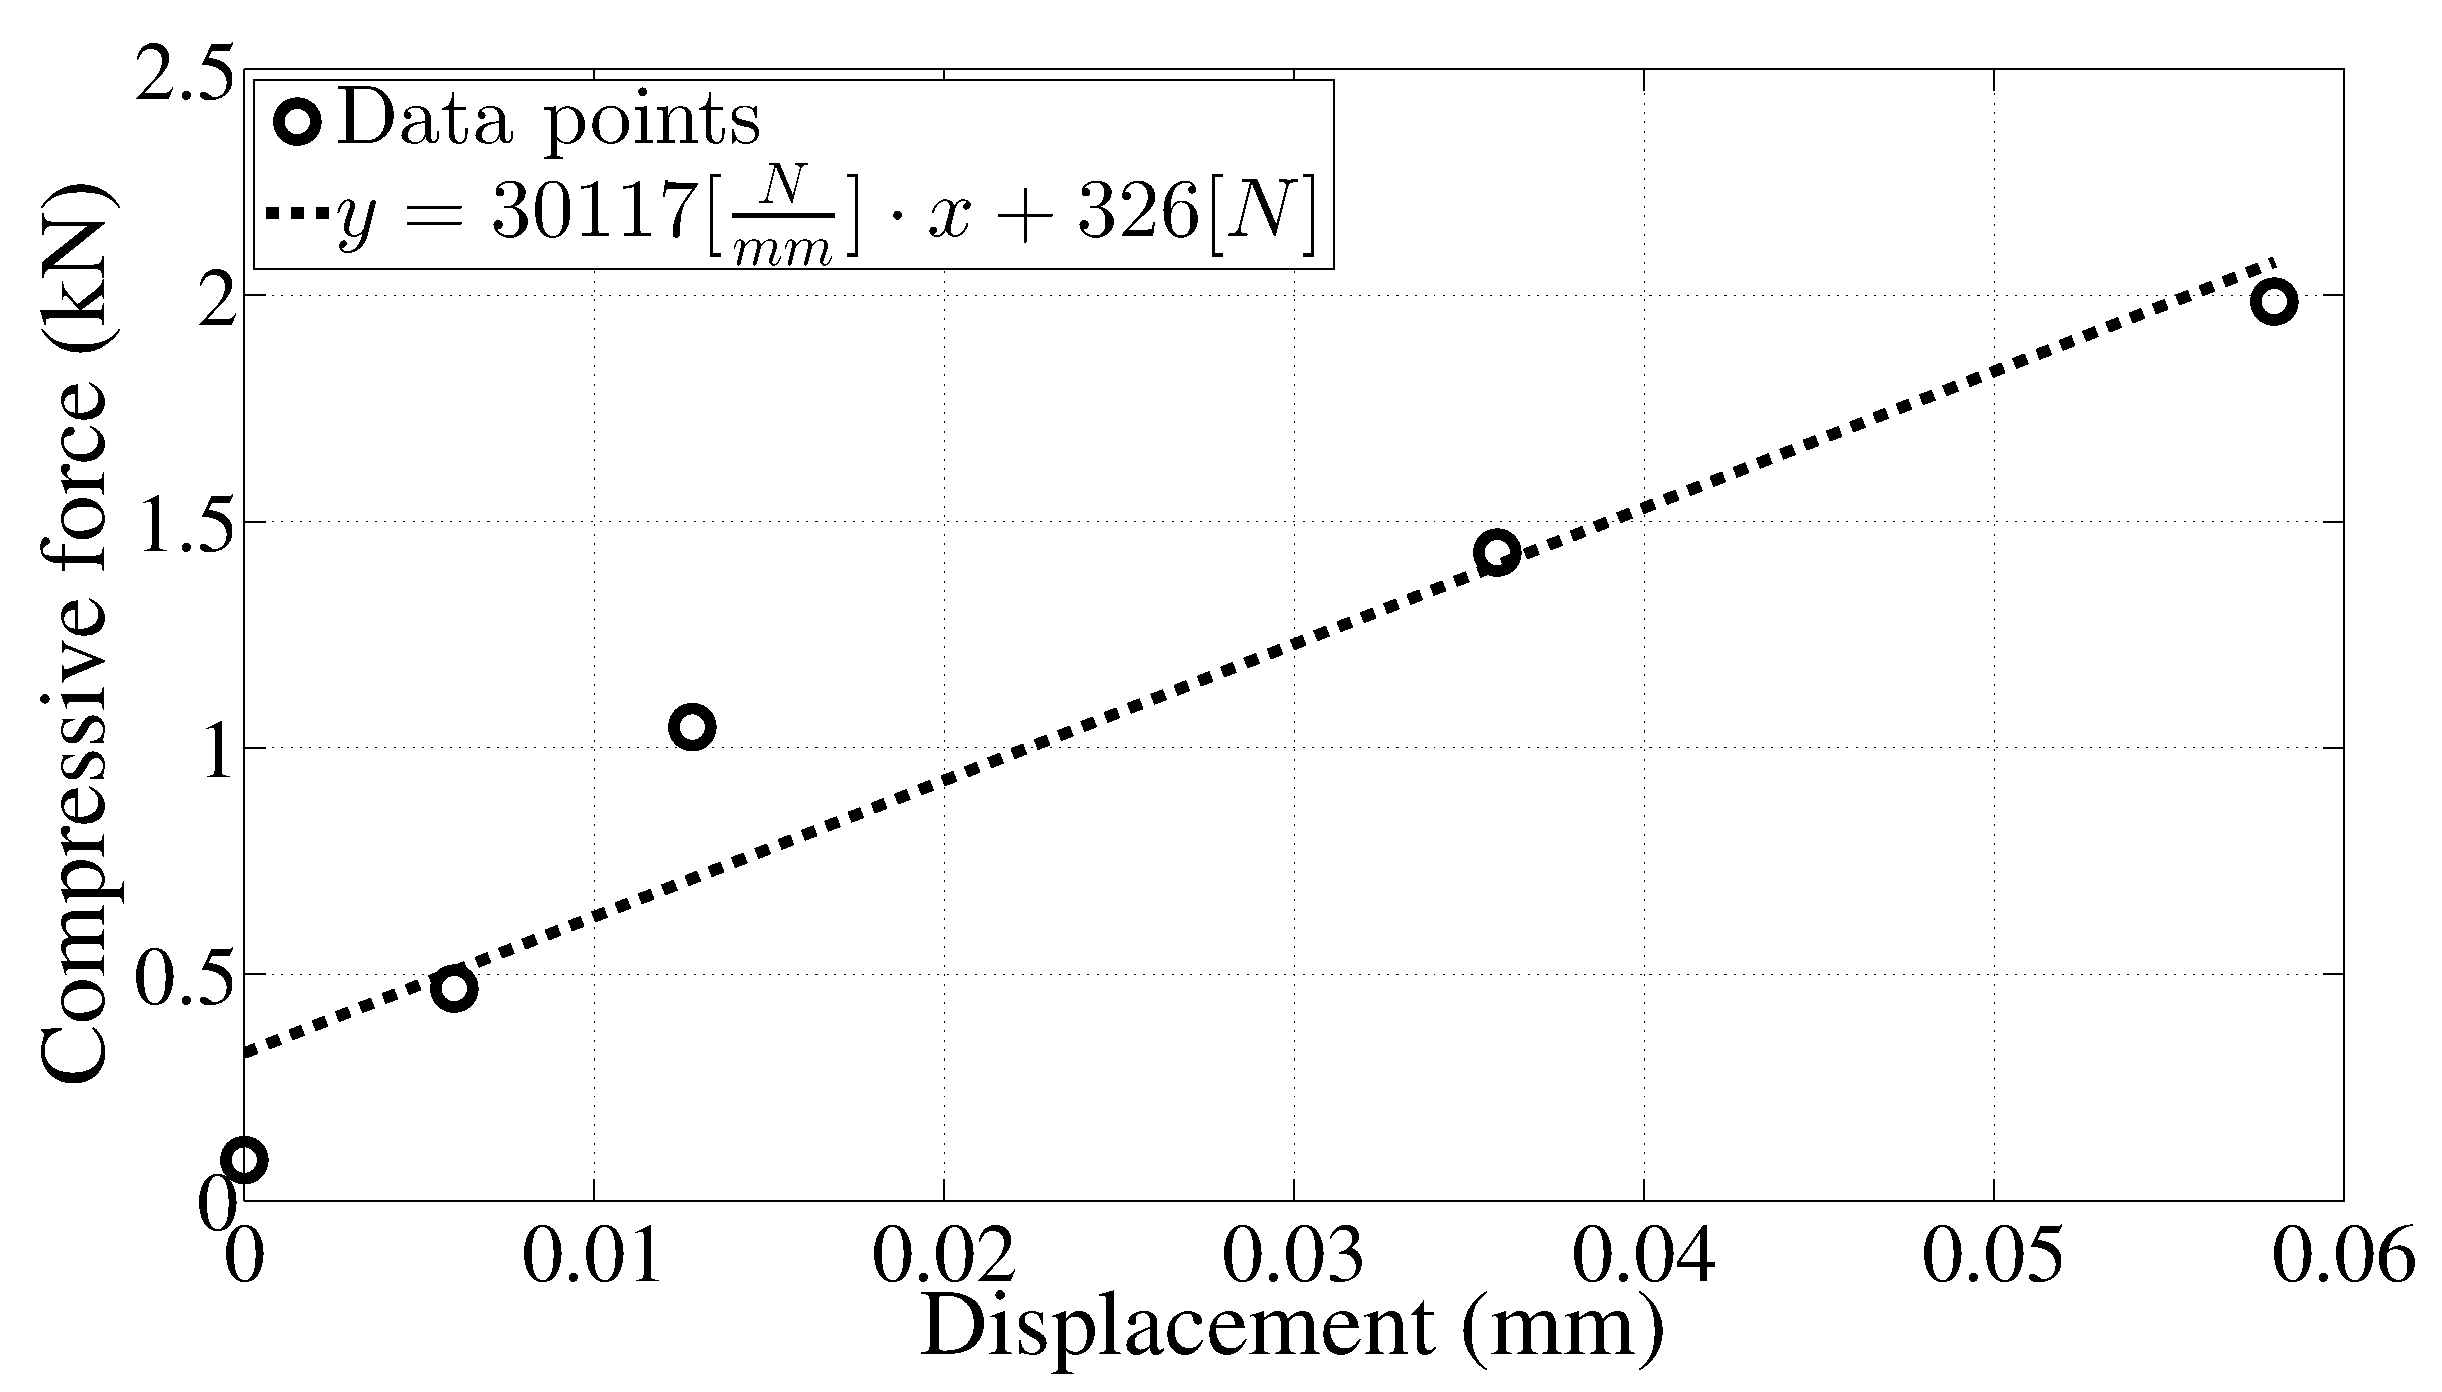
\includegraphics[width=\linewidth]{./appendixSupport/Figures/insComp}
\caption[Materials testing machine compliance results]{\textbf{The materials testing machine compliance tests showed a linear increase in displacement with force. The stiffness was calculated by fitting a line to the data.} Graphic \copyright Seth Gilchrist, 2013.}
\label{fig:insComp}
\end{figure}

\subsection{Drop tower compliance}
\label{sec:equipment_dt_compliance}
The drop tower is a linear impact device consisting of four vertical rails and a horizontal gantry.
It is constructed almost entirely out of 1$\frac{5}{8}$~inch strut-lock channel.
This design gives it great flexibility to be reconfigured, but the open cross section and friction-lock joints mean that as a foundation material it is quite compliant.
However using the static response is likely to overestimate the displacement in the initial seconds after an impact.
For this reason, a dynamic model of the structure was used to estimate the displacement-time profile during the impact.
This compliance could lead to potentially large displacements of the loading platform during impact.
To preform these calculations, two things needed to ne known, i) the compliance of the structure; ii) the mass mounted to the top of the structure.

\subsubsection{Methods}
To measure the compliance of the drop tower, a significant load needed to be applied and the displacement of the loading platform needed to be measured.
Unlike the materials testing machine, the drop tower does not have a way to apply a constant, high force to the platform, therefore, an external means of applying the force was used.
A 50~gallon barrel was placed on top of the loading platform and filled with rocks to apply the load (Figure~\ref{fig:dtCompliance}).
A dial gauge was fixed to a platform sitting on the floor and oriented to measure vertical displacement using a laser level.
The drop tower's single axis load cell (LC 402, Omega Engineering, Stamford, CT) was used to measure compressive loads.
Rocks were used from dead weight and were transferred into the barrel and load and displacement readings were taken at 500~\ac{n} intervals.
Measurements were taken during loading and unloading and the stiffness of the machine was determined by averaging the slopes of the loading and unloading curves.

After unloading the drop tower, the loading platform was removed along with the T-slot plate, load cell and all other mounting apparatus down to the strut-lock channel foundation.
These items were weighed using a digital scale for items less than 20~\ac{kg} and an analogue bathroom-style scale for those over 20~\ac{kg}.

\begin{figure}
\centering
\begin{subfigure}[b]{0.3\textwidth}
\includegraphics[width=\textwidth]{./appendixSupport/Figures/dtAndRocks}
\caption{Before}
\label{fig:dtCompBefore}
\end{subfigure}
~
\begin{subfigure}[b]{0.3\textwidth}
\includegraphics[width=\textwidth]{./appendixSupport/Figures/dtFullRocks}
\caption{After}
\label{fig:dtCompAfter}
\end{subfigure}
~
\begin{subfigure}[b]{0.3\textwidth}
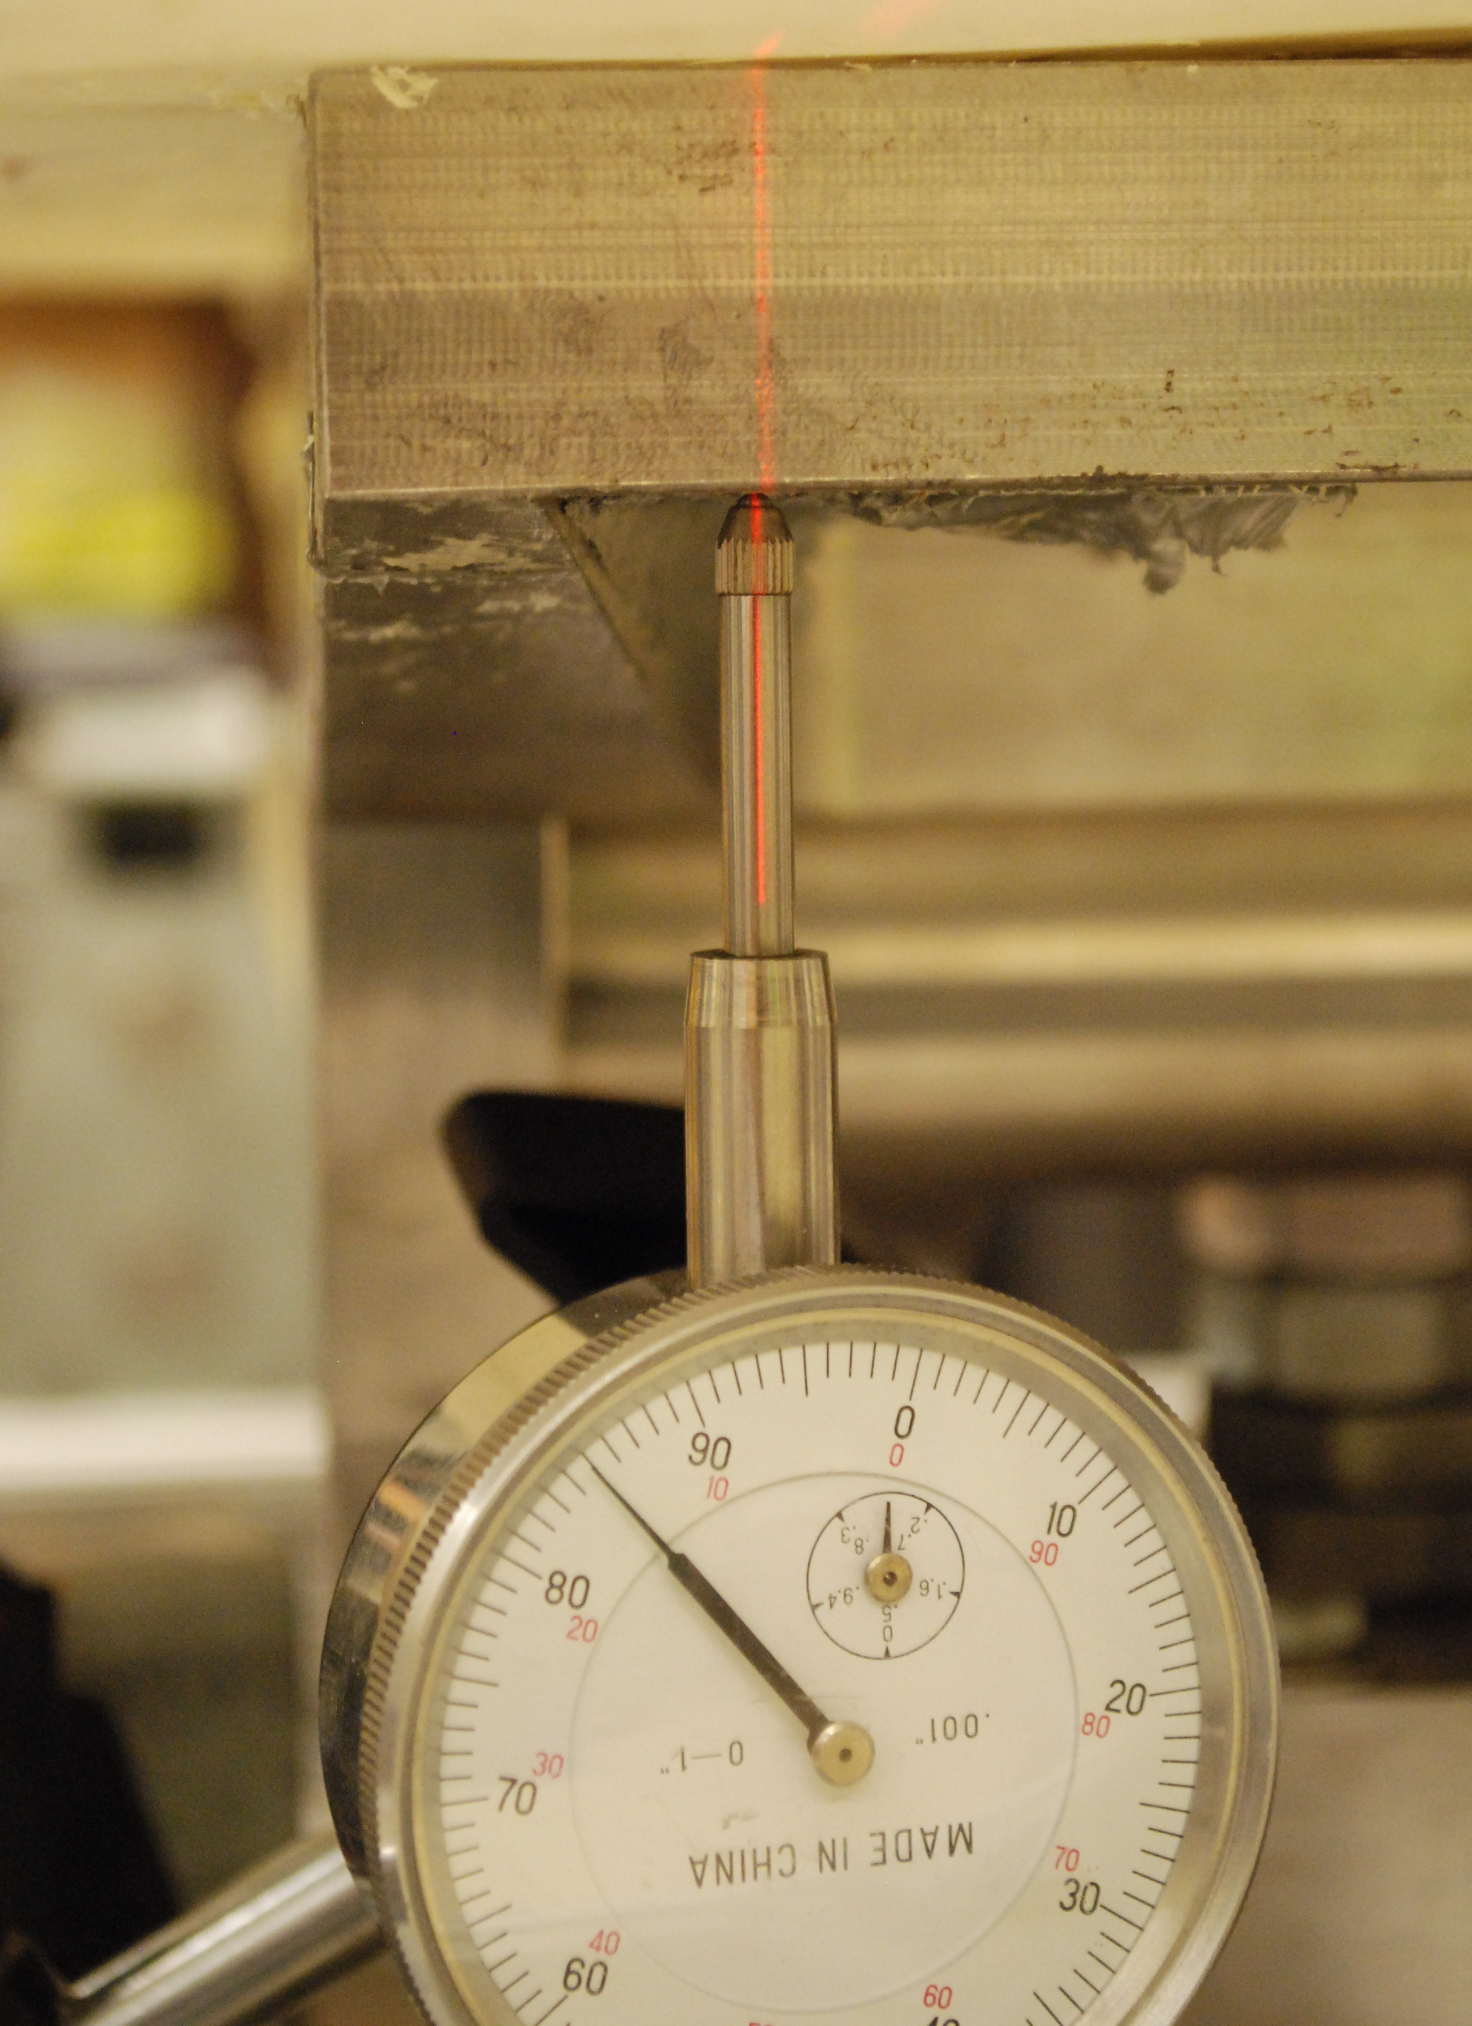
\includegraphics[width=\textwidth]{./appendixSupport/Figures/dtDialGauge}
\caption{Dial gauge}
\label{fig:dtCompDialGauge}
\end{subfigure}
\caption[Drop tower compliance test]{\textbf{The drop tower was loaded using a barrel filled with rocks. The displacement of the loading platform was measured using a dial gauge which was referenced to the ground.} Graphic \copyright Seth Gilchrist, 2013.}
\label{fig:dtCompliance}
\end{figure}

\subsubsection{Results}
The drop tower showed linear behaviour during loading and unloading (Figure~\ref{fig:dtComp}).
The stiffness varied by 13\% between loading and unloading.
This change in stiffness is likely due to the hysteresis of the friction joints at junctions in the strut-lock channel.
The average stiffness for combined loading and unloading was 5637~\ac{n}/\ac{mm}.

\begin{figure}
\centering
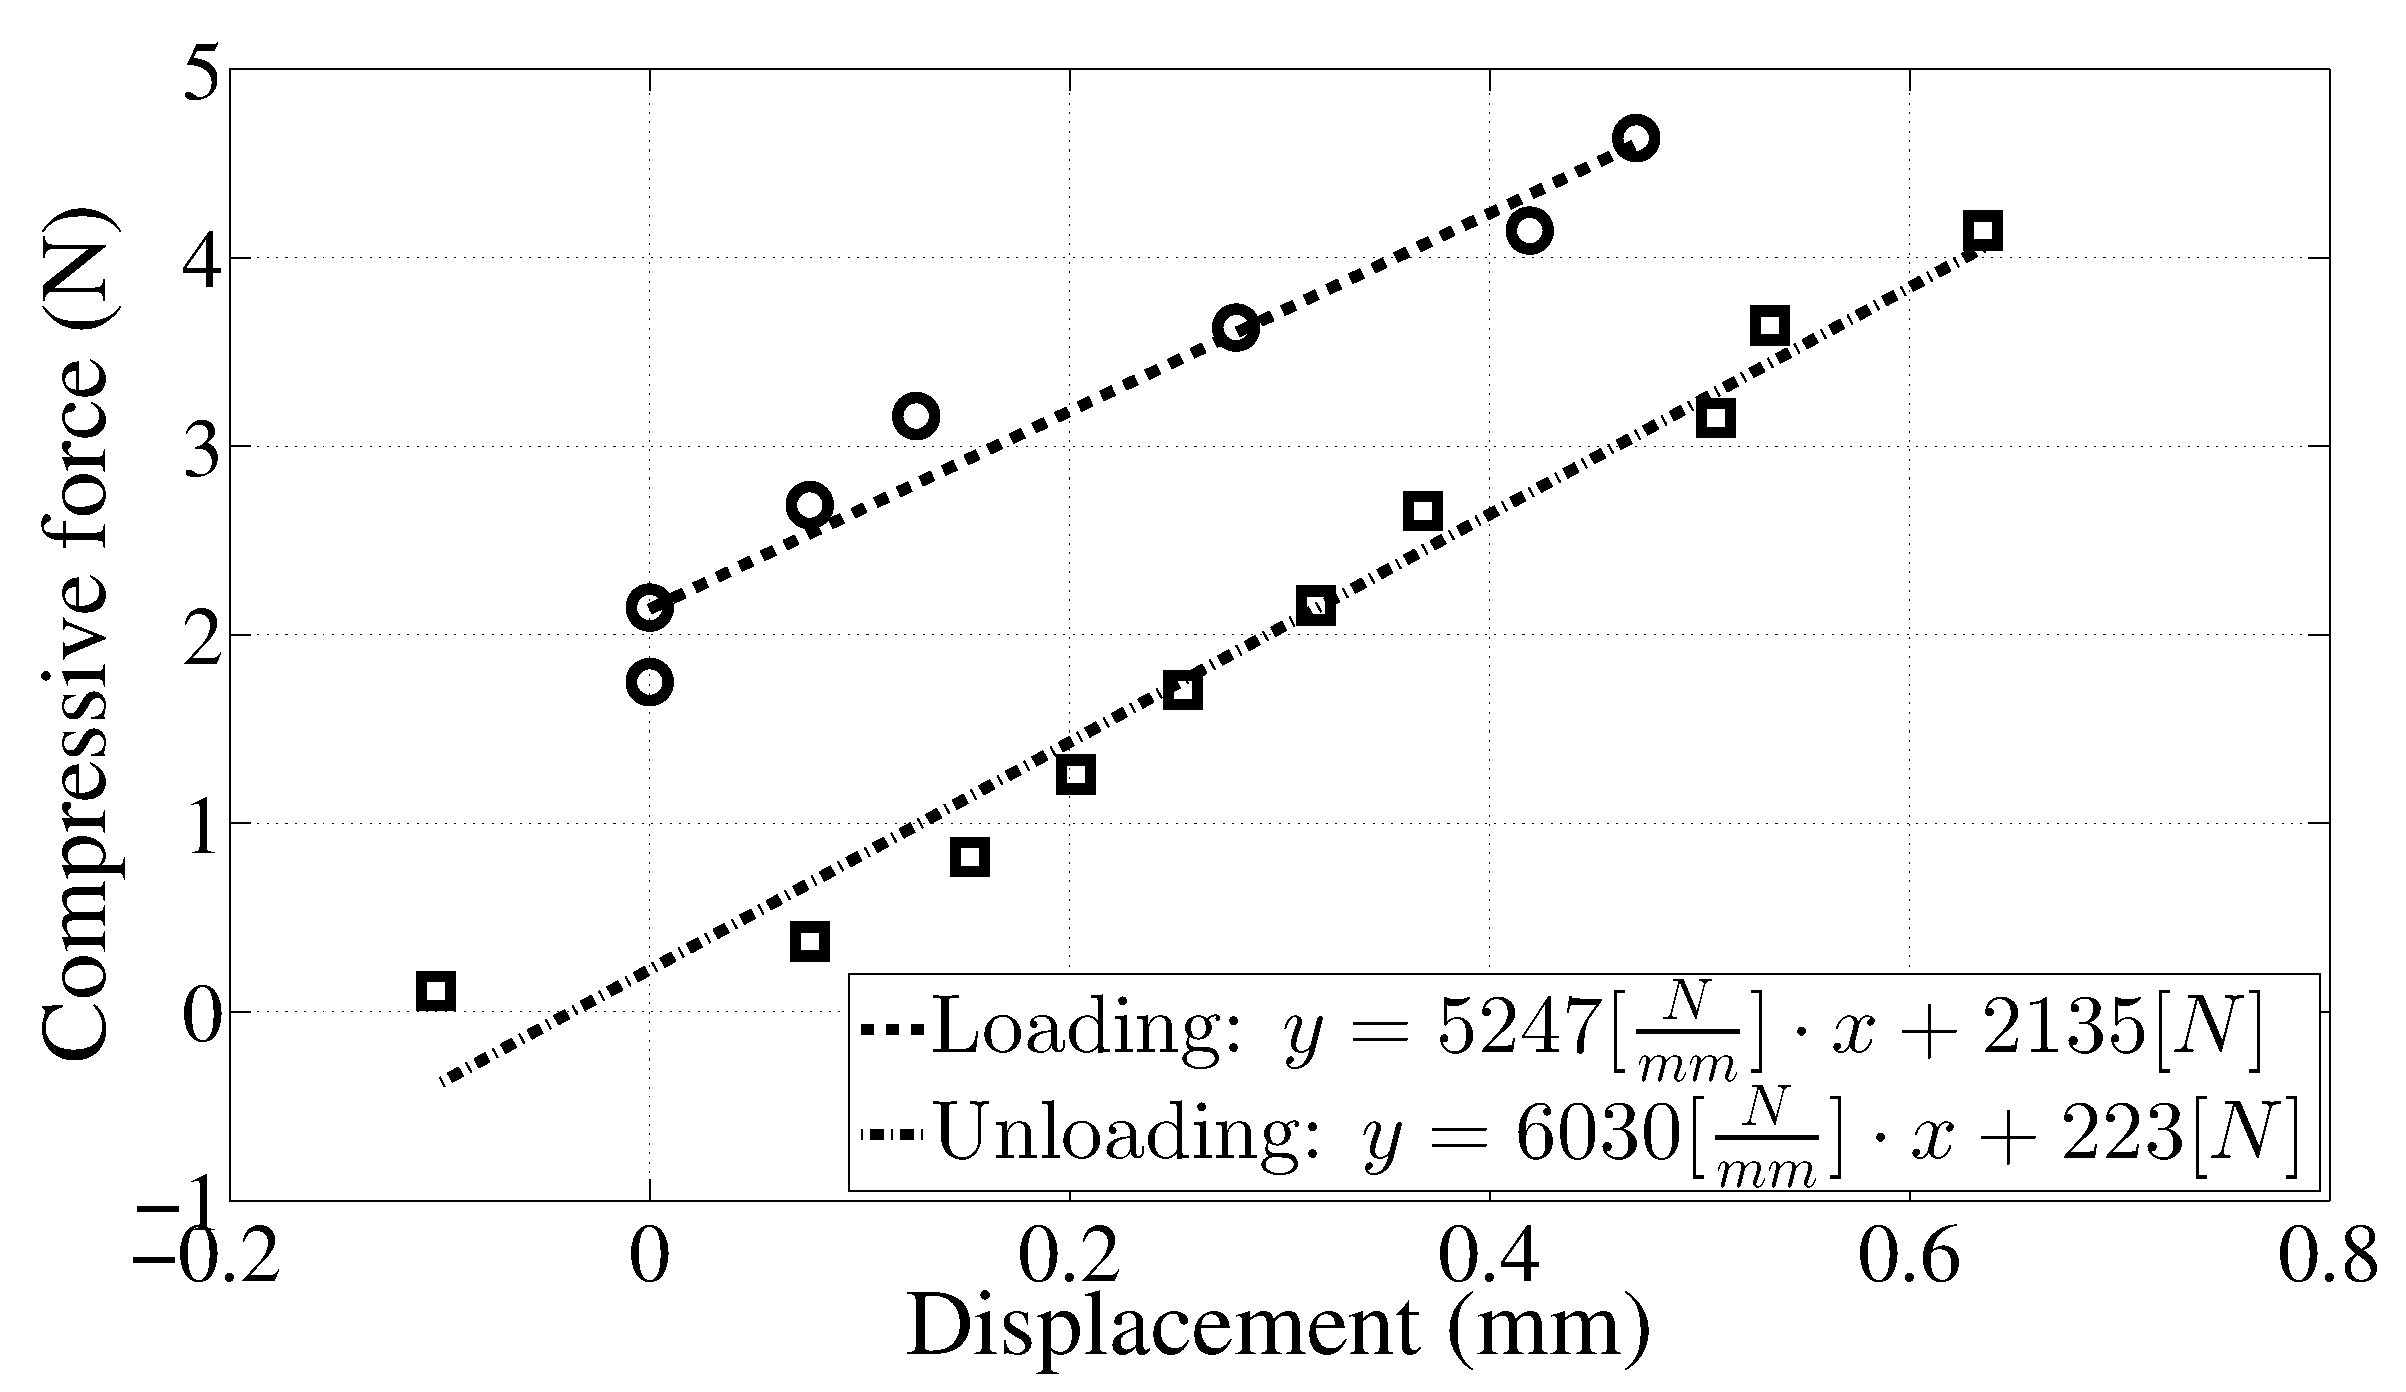
\includegraphics[width=\linewidth]{./appendixSupport/Figures/dtComp}
\caption[Drop tower compliance results]{\textbf{The drop tower showed linear behaviour during both loading and unloading.} Graphic \copyright Seth Gilchrist, 2013.}
\label{fig:dtComp}
\end{figure}

\begin{table}
\centering
\caption[Drop tower apparatus mass]{Mass of all all test apparatus used in the drop tower.}
\label{tab:equipment_dt_mass}
\begin{tabularx}{0.5\textwidth}{>{\raggedright\arraybackslash}X >{\raggedleft\arraybackslash}X}
\toprule
Item & Mass (\ac{kg}) \\
\midrule
Loading platen & 23.18 \\
Load cell & 6.419 \\
T-slot plate & 21.36 \\
Bearing plates & 1.896 \\
Head support plates & 2.327 \\
Mount plate & 13.66 \\
Bottom plate & 14.54 \\
Pivot rod & 0.507 \\
\textbf{Total} & \textbf{83.89}\\
\bottomrule
\end{tabularx}
\end{table}

\subsection{Foam compliance}
\label{sec:equipment_foam}
The foam used to pad the greater trochanter was bought from a local Evazote\textsuperscript{\textregistered} supplier.
Foams can be prone to variations in material properties because of the complexity of the manufacturing process.
For this reason, an experiment was performed to measure the foam's compliance at different levels of compression.

\subsubsection{Methods}
A 2~inch square piece of foam was cut from the same sheet of foam used in the fall simulation tests.
The foam was loaded into the materials testing machine (8874, Instron, Noorwood, MA) an compressed to 75\%, 50\% and 25\% of its original height in displacement control.
Compressive force measurements were taken at each level of compression.
Stiffness was defined as the average stiffness to the compression level under inspection.

\subsubsection{Results}
The stiffness was seen to increase by a power-law relationship as compression increased (Table~\ref{tab:equipment_foam_compression}).
The stiffness was relatively constant between the 25\% and 50\% compression measurements, but as the foam pores collapsed a sharp increase in stiffness was observed.

\begin{table}
\centering
\caption[Foam stiffness and stress]{Nominal stiffness and stress in the foam at various compression levels.}
\label{tab:equipment_foam_compression}
\begin{tabularx}{0.75\textwidth}{>{\centering\arraybackslash}X >{\centering\arraybackslash}X >{\centering\arraybackslash}X}
\toprule
Compression(\%) & Stress (\acs{kpa}) & Stiffness (\acs{kn}/\acs{m}) \\
\midrule
25 & 36 & 19.92 \\
50 & 95 & 26.45 \\
75 & 308& 57.39 \\
\bottomrule
\end{tabularx}
\end{table}

\subsection{Drop tower position measurement verification}
\label{sec:equipment_position}
The positions of the greater trochanter and impact hammer were measured using image tracking techniques.
This technique involved videoing the impact hammer and the greater trochanter during the impact event and using TEMA Automotive (v3.0, Image Systems, North Hollywood, CA) to measure the displacements.
Frames from the video were loaded input TEMA and an image of a calibration target was used to correct the images for lens distortion.
Tracking was done using a 1~\ac{cm} square target on the impact hammer, and the junction of the bone and \acf{pmma} potting cap.

\subsubsection{Methods}
To determine the accuracy of this measurement, the impact hammer used in the fall simulation tests was secured in a materials testing machine (8874, Instron, Noorwood, MA).
A piece of surrogate bone with a similar colour to human bone was secured to the impact hammer using the same \ac{pmma} used in the fall simulation testing.
The camera and lens used in the fall simulation tests were set up at the same distance, focal length, focus and frame rate as in the fall simulation tests.
Lighting was also adjusted to be similar to the fall simulation tests.
A dial gauge was arranged to measure the displacement of the impact hammer to confirm the displacement reported by the TEMA and Instron software.
A second camera was arranged to record the dial gauge during the test and spot comparisons were made between the Instron output and dial gauge reading.
A \acl{daq} was used to record the output of the materials testing machine and the camera trigger signal to synchronize the readings.
The materials testing machine was programmed to move the cross head according to the equation $5\sin(10\pi t)$~\ac{mm}, which gives a maximum velocity of 157~\ac{mm}/\ac{s}.

\subsubsection{Results}
The Instron output and dial gauge showed good correlation.
Ten spot checks showed an average(\ac{sd}) difference of -0.10(0.06)~\ac{mm} (Table~\ref{tab:equipment_position}).
The comparison of the TEMA with the Instron also showed good correlation, with an average(\ac{sd}) error of -0.032(.043)~\ac{mm} (Figure~\ref{fig:PlotInsTEMA}).

\begin{table}
\centering
\caption[Materials testing machine position verification]{Values and differences of the materials testing machine and dial gauge at various times}
\label{tab:equipment_position}
\begin{tabular}{l c c c }
	\toprule
	Time post trigger (\ac{ms}) & Dial gauge (\ac{mm}) & Instron (\ac{mm}) & Difference (mm) \\ \midrule
	64.643                      & 4.928         & 5.080              & -0.152 \\
	114.771                     & 9.906          & 10.025           & -0.119 \\
	164.790                      & 4.851         & 4.942            & -0.091 \\
	189.528                     & 1.397          & 1.389            & 0.008 \\
	253.435                     & 3.175          & 3.334            & -0.159 \\
	276.437                    & 6.731          & 6.870            & -0.139 \\
	292.821                     & 8.763          & 8.918            & -0.155 \\
	364.214                     & 4.953          & 5.030            & -0.077 \\
	381.140                      & 2.413          & 2.440            & -0.027 \\ 
\multicolumn{3}{r}{\textbf{Average}}								 & \textbf{-0.101} \\
\multicolumn{3}{r}{\textbf{Standard Deviation}}						 & \textbf{ 0.060} \\
\bottomrule
\end{tabular}
\end{table}

\begin{figure}
\centering
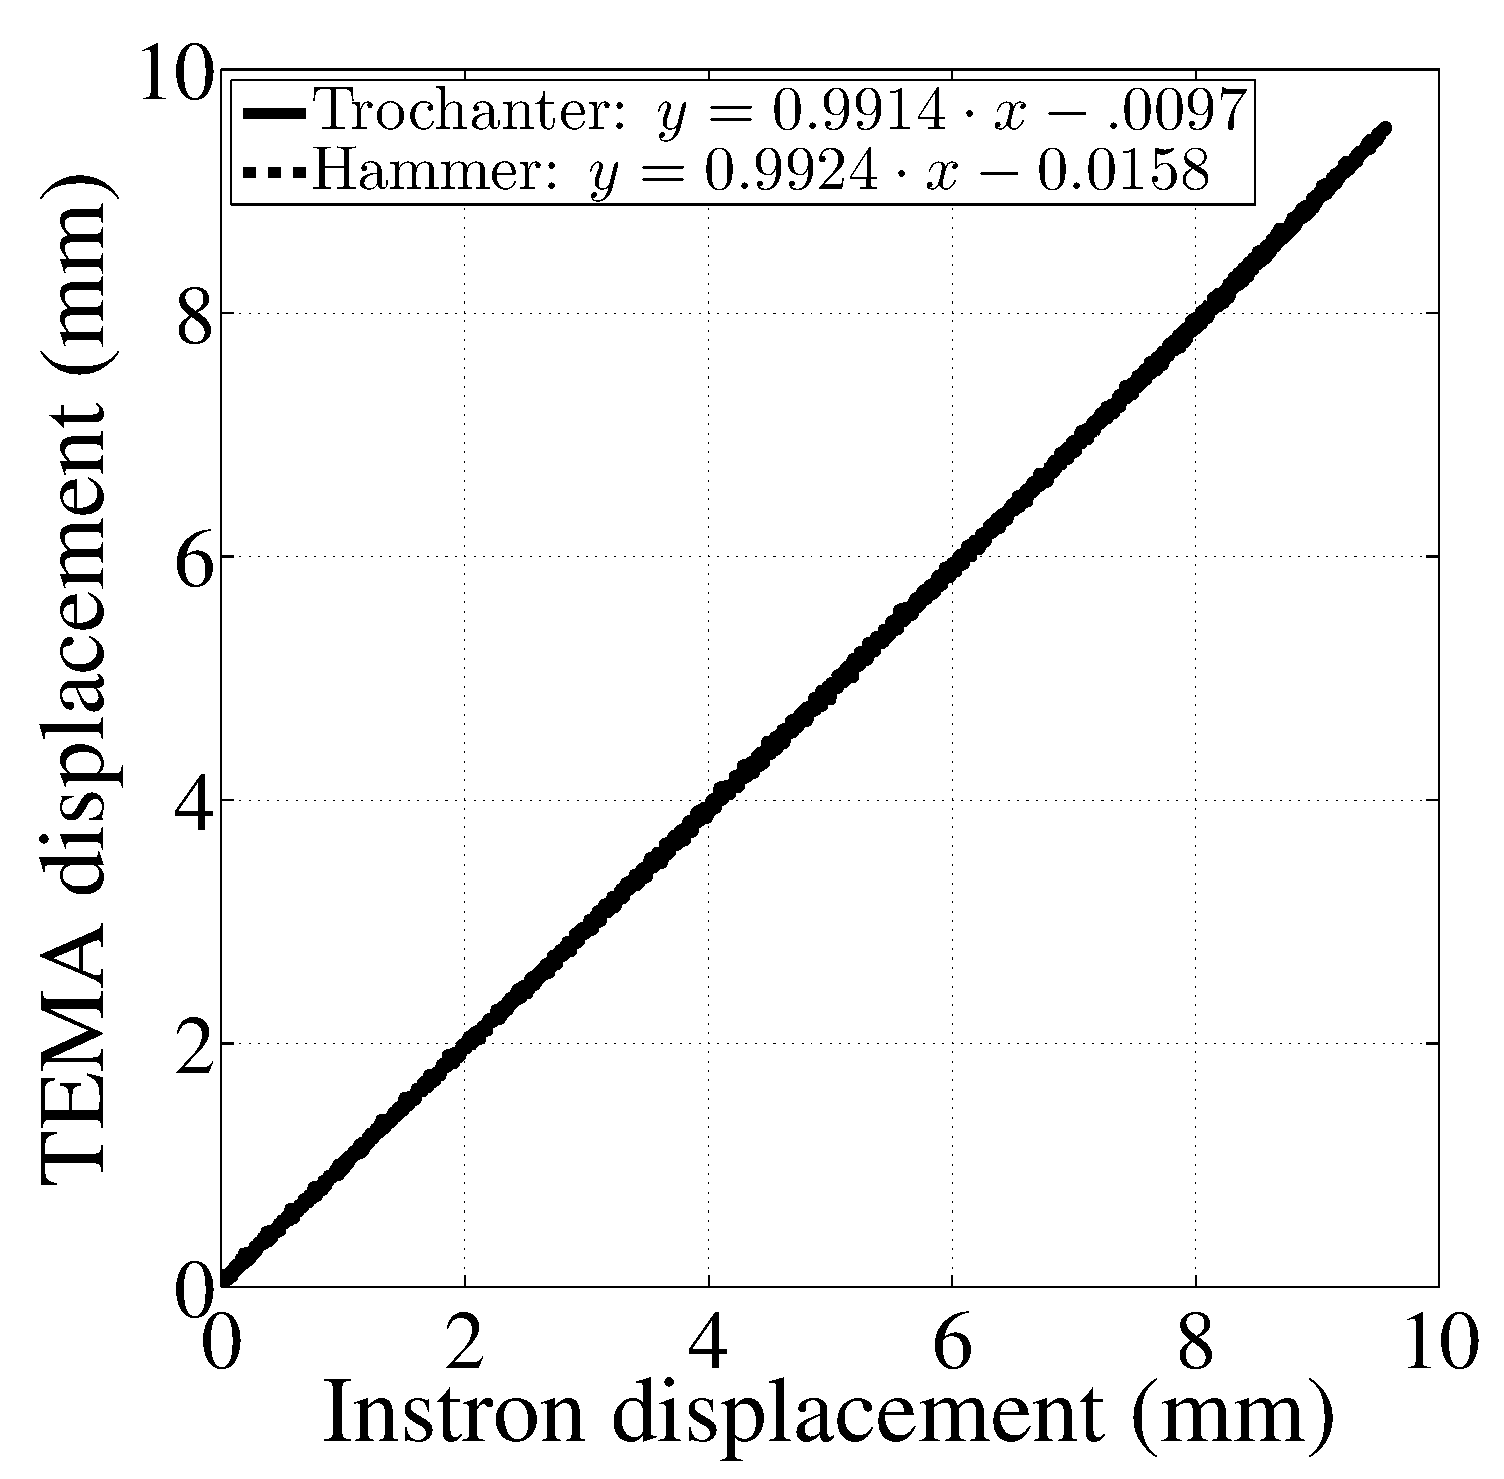
\includegraphics[width=0.55\linewidth]{./appendixSupport/Figures/PlotInsTEMA}
\caption[TEMA measured displacement verification]{\textbf{The displacement measured by TEMA for both the trochanter and the impact hammer agreed well with each other and with the output of the materials testing machine. In this plot the lines are coincident and as such impossible to differentiate.} Graphic \copyright Seth Gilchrist, 2013.}
\label{fig:PlotInsTEMA}
\end{figure}
